
\newcommand{\dAe}   {\ensuremath{d_A^\epsilon}}
\newcommand{\dApe}  {\ensuremath{d_A^{+\epsilon}}}
\newcommand{\tdAe}  {\ensuremath{\tilde{d}_A^\epsilon}}
\newcommand{\tdApe} {\ensuremath{\tilde{d}_A^{+\epsilon}}}
\newcommand{\triP}  {\ensuremath{\tau_P}}
\newcommand{\triQ}  {\ensuremath{\tau_Q}}
\newcommand{\triPP} {\ensuremath{\tau'_P}}
\newcommand{\triQQ} {\ensuremath{\tau'_Q}}

\begin{figure}[t]
\centering

\psfrag{A}{$A$}
\psfrag{Ap}{$A'$}
\psfrag{B}{$B$}
\psfrag{p}{$p$}
\psfrag{q}{$q$}

\begin{tabular}{cc}
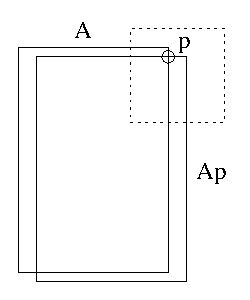
\includegraphics[width=0.4\linewidth]{images/rectA.eps} \qquad &
\qquad
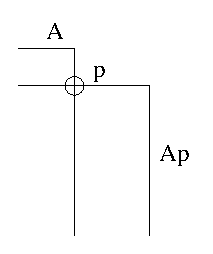
\includegraphics[width=0.4\linewidth]{images/rectAclose.eps} \\
(a) & (b) \\
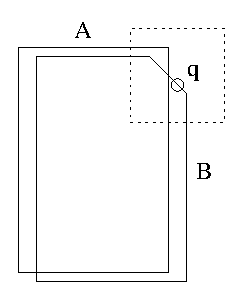
\includegraphics[width=0.4\linewidth]{images/polyB.eps} \qquad &
\qquad
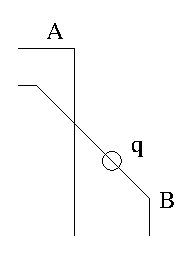
\includegraphics[width=0.4\linewidth]{images/polyBclose.eps} \\
(c) & (d)
\end{tabular}

\caption{(a) Rectangle $A'$ is a slight perturbation of rectangle $A$.
(b)~Close up view of dotted region around point $p$.
(c) The corner of polygon $B$ is clipped near $q$.
(d)~Close up view of dotted region around point $q$.}
\label{fig:rect}

\end{figure}


\section{Measuring Angular Distance between Surfaces}
\label{section:angular_distance}

As described in Section~\ref{section:related},
we evaluated MergeSharp in~\cite{bw-cisec-13}
by extracting sharp mesh edges (dihedral angle less than $140^\circ$)
and comparing the 1-skeleton formed
by those sharp edges with the 1-skeleton of the sharp edges 
in an ideal surface.
We present here a different way of evaluating 
a reconstructed mesh containing sharp features.

Let $\Sigma_P$ and $\Sigma_Q$ be two surfaces.
Given a point $p \in \Sigma_P$,
the distance, $d(p,\Sigma_Q)$, from $p$ to $\Sigma_Q$
is the distance from $p$ to the closest point on $\Sigma_Q$,
i.e., $d(p, \Sigma_Q) = min_{q \in \Sigma_Q} d(p,q)$.
We would like a similar measurement of the difference between
the normal at $p$ and the normals of $\Sigma_Q$.

The simplest approach would be to locate the point $q \in \Sigma_Q$
closest to $p$ and measure the difference 
between their normals.
As shown in Figure~\ref{fig:rect},
this measurement is not be very useful.
Rectangle $A'$ is a slightly translation of rectangle $A$.
The boundaries of rectangles $A$ and $A'$
are close under the Hausdorff metric and their normals are the same.
However, point $p$ is in the intersection of the two boundaries,
$\partial A$ and $\partial A'$,
but the normal to point $p$ in $\partial A$ is $90^\circ$
from the normal to point $p$ in $\partial A'$.
Furthermore, for any point $\tp \in A$ in a suitably small neighborhood of $p$,
the closest point in $\tp' \in A'$ has normal which is $90^\circ$
from the normal of $A$ at $\tp$.
Note that the translation could be arbitrarily small
and there would still be a point in $A$ whose normal was $90^\circ$
from the closest point in $A'$.

In contrast to the match between the normals of $A$ and $A'$, 
the corner of polygon $B$ in Figure~\ref{fig:rect}(c)
is clipped and its normal is $45^\circ$ from any normal of $A$.
We would like some measurement which gives a high value 
between $q \in B$ and $A$ while giving a low value between
any point of $A'$ and $A$.
Our idea is to compare the normal at $p \in \Sigma_P$ 
with the normals of $\Sigma_Q$ in some suitable neighborhood 
around $p$.

Let $\Sigma^S_P$ and $\Sigma^S_Q$ be the set of smooth points
in $\Sigma_P$ and $\Sigma_Q$.
Let $n_p$ and $n_q$ be the normals of $p \in \Sigma^S_P$
and $q \in \Sigma^S_Q$, respectively.
Let $B_p(\epsilon)$ be the ball around $p$ of radius $\epsilon$.
For each point $p \in \Sigma^S_a$ 
where $B_p(\epsilon) \cap \Sigma^S_Q \neq \emptyset$,
define the angle distance between $p$ and $\Sigma_Q$
in the neighborhood $\epsilon$ as:
\begin{align*}
\tdAe(p,\Sigma_Q) & = \liminf\{ \angle(n_p, n_q) : 
q \in \Sigma^S_Q \cap B_p(\epsilon) \}.
\end{align*}

Define the directed angle distance between $\Sigma_P$ and $\Sigma_Q$
in neighborhood $\epsilon$ as:
\begin{align*}
\tdAe(\Sigma_P,\Sigma_Q) & = 
  \limsup_{p \in \Sigma^S_P \mbox{ and } 
  B_p(\epsilon) \cap \Sigma^S_Q \neq \emptyset} 
         \tdAe(p,\Sigma_Q).
\end{align*}

Finally, define the angle distance between $\Sigma_P$ and $\Sigma_Q$
in neighborhood $\epsilon$ as:
\begin{align*}
\dAe(\Sigma_P,\Sigma_Q) & = 
\max(\tdAe(\Sigma_P,\Sigma_Q), \tdAe(\Sigma_Q,\Sigma_P)).
\end{align*}

The angle distance depends upon the parameter $\epsilon$.
If some point $p \in \Sigma^S_P$ is not within $\epsilon$ of $\Sigma_Q$,
then $\tdAe(p,\Sigma_Q)$ is undefined.
To address this problem, we replace the neighborhood $B_p(\epsilon)$
by an extended neighborhood $B_p(\epsilon+d(p,\Sigma_q))$
where $d(p,\Sigma_q)$ is the distance from $p$ to $\Sigma_Q$.
The ball around $p$ is now guaranteed to intersect $\Sigma_Q$.

Define the angle distance 
between $p \in \Sigma^S_p$ and $\Sigma_Q$ in the extended
neighborhood $\epsilon$ as:
\begin{align*}
\tdApe(p,\Sigma_Q) & = 
  \liminf\{ \angle(n_p, n_q) : 
     q \in \Sigma^S_Q \cap B_p(\epsilon+d(p,\Sigma_Q)) \}.
\end{align*}
As before, $d(p,\Sigma_Q)$ is the distance from $p$ to the closest point on $Q$.
Note that the addition of $d(p,\Sigma_Q)$ ensures that the ball
around $p$ intersects $\Sigma_Q$.

Define the directed angle distance between $\Sigma_P$ and $\Sigma_Q$
in extended neighborhood $\epsilon$ as:
\begin{align*}
\tdApe(\Sigma_P,\Sigma_Q) & = \limsup_{p \in P_S} \tdApe(p,\Sigma_Q).
\end{align*}

Define the angle distance between $\Sigma_P$ and $\Sigma_Q$
in extended neighborhood $\epsilon$ as:
\begin{align*}
\dApe(\Sigma_P,\Sigma_Q) & = 
\max(\tdApe(\Sigma_P,\Sigma_Q), \tdApe(\Sigma_Q,\Sigma_P)).
\end{align*}

Unfortunately, neither $\dAe(\Sigma_p, \Sigma_q)$
nor $\dApe(\Sigma_p, \Sigma_q)$ obey the triangle inequality.
Nevertheless, we think that the angle distance is a useful way
of measuring the difference in surface normals between two surfaces.


